\documentclass{article}

\usepackage{graphicx, amsmath}

\begin{document}

\title{Ordinal Data clustering and prediction}


TODO:

1. add review of proportinal odds approach

2. ordered stereotyp model is one of finite mixture modeling (update to review)

3. add math for  these two model

\author{Quan Zhao}

\maketitle

% \begin{abstract}
% \textbf{If you need an abstract, then it goes here. While you are reading this document, please also criticise it for the writing style, grammar, consistency, suitability, etc. }
% \end{abstract}

% 1. Search for relevant literature - 0:30
% 2. Evaluate and select sources -  0:58
% 3. Identify themes, debates, and gaps - 1:26
% 4. Outline your literature review's structure - 1:56
% 5. Write it - 2:34

\section{Introduction}
% introduction of the research topic
% (1/2 to 1 page).

% Finite mixture models are a flexible and powerful tool in statistical analysis, offering several key features that contribute to their widespread use in various fields.  These models assume that the observed data are generated from a combination of different probability distributions, each representing a distinct subpopulation within the overall population. The term "finite" in finite mixture models refers to the specific number of components or subpopulations in the mixture.

% Figure~\ref{fig:trend} shows the finite mixture modelling has strong trend in publications.

% intro of Ordinal Data

\subsection*{Ordinal Data}

Ordinal data is a type of categorical data in statistics that represents categories with a meaningful order or ranking among them, but without a precise difference in the scale between each category. This type of data is distinct because, while it allows for a rank order among the values, the intervals between the values are not necessarily equal or known. This means that ordinal data can tell us about the order of categories but not about the magnitude of difference between them.

Ordinal data include, Ranking data which can be sorted or ranked in order, but the distances between data points are not meaningful.
Ordinal data often consists of labels or descriptions, though it can be coded with numbers for analysis. Even when numerical codes are used, arithmetic operations (such as addition or subtraction) are not meaningful.
Statistical analysis of ordinal data typically involves non-parametric methods. The median and mode can be used as measures of central tendency

Ordinal data is common in surveys, questionnaires, and other forms of qualitative research, where it's used to capture attitudes, opinions, preferences, and other subjective assessments that inherently have an order but not a measurable distance between categories. 

Ordinal data are the most frequently encountered type of data in the social
sciences. Survey data, in which respondents are asked to characterize their opinions
on scales ranging from “strongly disagree” to “strongly agree,” are a common
example of such data. For our purposes, the defining property of ordinal data
is that there exist a clear ordering of the response categories, but no underlying
interval scale between them. For example, it is generally reasonable to assume an
ordering of the form
strongly disagree < disagree < dont know < agree < strongly agree,
but it usually does not make sense to assign integer values to these categories.
Thus, statements of the type
\[
\text{``disagree''} - \text{``strongly disagree''}
\]

\[
\text{``agree''} - \text{``don't know''}
\]
are not assumed. (Johnson, 2006~\cite{Johnson1999})

\subsection*{Difference to continuous data}

In the context of statistical analysis, the distinction between ordinal and continuous data types is pivotal, influencing both the choice of analytical methods and the depth of insights that can be derived. 
Ordinal data, characterized by its capacity to rank order categories without indicating precise differences between them, is inherently less informative than continuous data. 
Continuous data, with its quantitative nature, allows for an infinite range of values and supports detailed statistical operations, including arithmetic calculations and the application of advanced statistical models, facilitating a nuanced understanding of variables and their interrelations (Stevens, 1946~\cite{Stevens1946}).

The limitations of ordinal data stem from its inability to quantify the exact magnitude of differences between categories, a factor that restricts the application of parametric statistical methods. This constraint necessitates reliance on non-parametric methods, focusing on medians and modes rather than means and standard deviations, thereby offering a less detailed analysis (Conover, 1999~\cite{Conover1999}). 
For instance, in Likert scale responses commonly used in surveys, the ordinal nature of data precludes meaningful calculations of averages or differences between responses, limiting the depth of analysis that can be achieved (Likert, 1932~\cite{Likert1932}).

Comparatively, continuous data's capacity for precise measurement and the application of a broader range of statistical analyses enables a more detailed and accurate exploration of phenomena. This difference underscores the importance of data type consideration in research design and analysis, as it directly impacts the validity and comprehensiveness of research findings.

In summary, while ordinal data is invaluable for capturing rankings and subjective assessments, its analytical limitations highlight the superior informational value of continuous data in quantitative research. This distinction is crucial for researchers in the selection of appropriate statistical methods and in the interpretation of their data, ensuring that conclusions drawn are both valid and meaningful.

% clustering

\section{Statistical based Ordinal Data Clustering}

\subsection{Finite Mixture modeling}

Finite mixture models have emerged as a versatile and powerful statistical tool, garnering increasing attention across various scientific and research disciplines. These models, predicated on the assumption that observed data arise from a blend of several probability distributions, each representing a distinct subpopulation, have revolutionized our approach to understanding complex data structures. The designation "finite" in finite mixture models is pivotal, indicating the specific, but variable, number of components or subgroups within the data. This finite aspect offers a balance between model complexity and interpretability, allowing for detailed yet manageable analysis of diverse datasets.

The significance of finite mixture models is vividly illustrated in Figure~\ref{fig:trend}, which showcases a robust upward trajectory in related publications. This trend not only reflects the growing academic and practical interest in these models but also underscores their evolving sophistication and broadening applicability. From the early advancements in maximizing likelihood estimation through algorithms like EM, as pioneered by McLachlan in 2000, to the more recent developments in handling a variety of data types, including binary, count, and ordinal data, finite mixture models have continuously adapted and expanded their scope.

\begin{figure}[ht!] % 'h!' places the figure here, in the text
    \centering % Centers the figure
    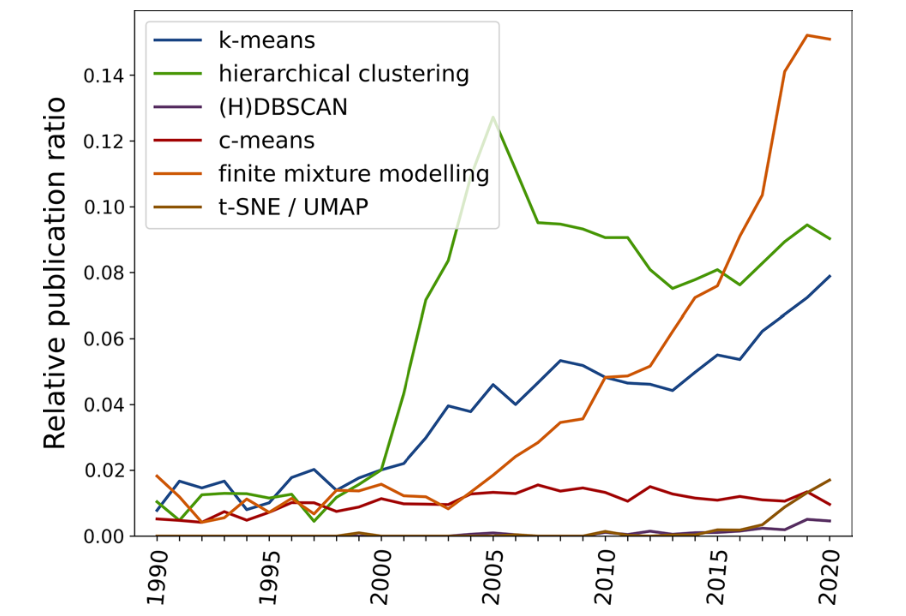
\includegraphics[width=0.6\textwidth]{images/trend.png} % Include the image with 50% of the text width
    \caption{The increase in publications indexed by PubMed that mention a keyword specific to cluster analyses relative to the number of publications 
    that mention a traditional statistical test. 
    Particularly sharp increases can be seen for finite mixture modelling.
    From~\cite{dalmaijer2022statistical}.} % Caption for the image
    \label{fig:trend} % Label for referencing the figure in the text
  \end{figure}

\subsection*{Early Developments (2000--2010)}

McLachlan's 2000 paper marked a crucial step in mixture model applications by simplifying the maximum likelihood estimation (MLE) using the EM algorithm. This approach, utilizing $Y_j$ and $Z_j$, not only enhanced the computational efficiency of MLE but also laid a foundational strategy for Bayesian approaches and MCMC methods in mixture models. The paper’s impact is evident in its widespread adoption across various domains, from bioinformatics to finance, where mixture models are employed (McLachlan, 2000~\cite{mclachlan2000finite}).

In 2002, Figueiredo's introduction of an unsupervised algorithm for learning finite mixture models was a game-changer. This method's ability to autonomously select the number of components represented a significant leap over previous techniques, which often relied on arbitrary or manual component selection. Additionally, the algorithm's robustness against initialization issues and singular estimates made it a go-to choice for practitioners dealing with complex multivariate data (Figueiredo, 2002~\cite{figueiredo2002unsupervised}).

A key paper in 2010 by Volodymyr and Ranjan addressed practical challenges in applying the EM algorithm for mixture models. This comprehensive guide to estimation, model selection, and likelihood maximization was a boon for both researchers and practitioners. Notably, the work extended beyond Gaussian mixtures, offering insights and methodologies for simulating and visualizing non-Gaussian mixtures, thereby broadening the applicability of mixture models (Volodymyr and Ranjan, 2010~\cite{10.1214/09-SS053}).

\subsection*{Recent Developments (2010--2019)}

In 2016, Matechou's proposal of finite mixture models for biclustering two-mode ordinal categorical data introduced a novel approach to data analysis. By employing proportional odds parameterization, these models provided a nuanced understanding of complex data patterns, useful in fields such as genomics and social sciences where ordinal data is prevalent. The utilization of the EM algorithm for model-fitting underscored the enduring relevance of this method in mixture model applications (Matechou, 2016~\cite{matechou2016biclustering}).

Fernandez in 2016 offered an alternative methodology for clustering ordinal data. The use of likelihood-based methods through finite mixtures with the stereotype model presented a robust framework for analyzing complex data structures. This approach was particularly notable for its application in fuzzy clustering techniques, an area of growing interest in data science (Fernandez, 2016~\cite{fernandez2016mixture}).

Jacques' 2018 introduction of a model-based co-clustering algorithm was a significant advancement. The algorithm's ability to handle missing data and its interpretability made it especially relevant for high-dimensional datasets. The BOS distribution employed in this model underscored the continuous innovation in probabilistic modeling techniques, catering to the increasing complexity of data in modern research (Jacques, 2018~\cite{jacques2018model}).

Fernandez's 2019 extension of finite mixture models to binary, count, and ordinal data under a unified statistical framework represented a consolidation and expansion of mixture model applications. The introduction of maximum likelihood estimation parameters and the Bayesian approach for simultaneous estimation were indicative of the field's progression towards more flexible and comprehensive modeling techniques (Fernandez, 2019~\cite{fernandez2019finite}).

\subsection*{Compare with other clustering algorithm}

Compare with Tree based or distance based clustering algorithm, statistical based clustering algorithm shows more powerful on ordinal data, especially for multiclass and multioutput case.
One reason is Ordinal data not assume the distance between each category are equal.
secondly, Ordinal data usually include few categories which not good for tree based regression.

\section{Conclusion and Future Directions}

The evolution of mixture models from McLachlan's initial work in 2000 to advanced models in 2019 showcases a field marked by dynamic growth and innovation. These models have not only solved historical challenges but also set the stage for future advancements. As the field progresses, a key focus is integrating machine learning with traditional statistical methods, enhancing the capability of mixture models to accurately predict cluster membership for new data points. This is especially relevant in artificial intelligence applications, where mixture models contribute to improved pattern recognition and decision-making.

Furthermore, as data complexity and volume continue to escalate, the demand for robust, efficient, and versatile mixture models is more critical than ever. Future research is expected to concentrate on scaling up these models and improving their adaptability across diverse data types and structures. This progression underscores the mixture models' indispensable role in modern data analysis, poised to address the ever-growing challenges in data science and AI.

\bibliographystyle{plain}
\bibliography{bibliography} % Replace 'yourbibfile' with the name of your .bib file


\end{document}

